\documentclass[12pt,a4paper]{article}

\usepackage{tikz}
\usepackage{array}
\usepackage{float}
\usepackage{times}
\usepackage{lipsum} % for lorem ipsum
\usepackage{amsmath}
\usepackage{amssymb}
\usepackage{caption}
\usepackage{graphicx}
\usepackage{geometry}
\usepackage{titlesec}
\usepackage{booktabs}
\usepackage{multirow}
\usepackage{setspace}
\usepackage{fancyhdr}
\usepackage{lastpage}
\usepackage{hyperref}
\usepackage{ragged2e} % for text alignment (justification)
\usepackage[utf8]{inputenc}
\usetikzlibrary{shapes.geometric, arrows, positioning}

% Glossaries
\usepackage[acronym]{glossaries}
\newacronym{ai}{AI}{Artificial Intelligence}
\newacronym{auc}{AUC}{Area Under the ROC Curve}
\newacronym{bbboa}{BBBOA}{Binary Brown Bear Optimization Algorithm}
\newacronym{bbo}{BBO}{Brown Bear Optimization}
\newacronym{ccf}{CCF}{Credit Card Fraud}
\newacronym{cgan}{CGAN}{Conditional Generative Adversarial Network}
\newacronym{cvae}{CVAE}{Conditional Variational Autoencoder}
\newacronym{dl}{DL}{Deep Learning}
\newacronym{dt}{DT}{Decision Tree}
\newacronym{dma}{DMA}{Data Mining Analytics}
\newacronym{dsm}{DSM}{Data Sampling Methods}
\newacronym{em}{EM}{Ensemble Methods}
\newacronym{ft}{FT}{Feature Transformation}
\newacronym{fa}{FA}{Fraud Analysis}
\newacronym{fs}{FS}{Feature Selection}
\newacronym{gan}{GAN}{Generative Adversarial Network}
\newacronym{gnn}{GNN}{Graph Neural Network}
\newacronym{gdp}{GDP}{General Discussion Placeholder} % optional, remove if unused
\newacronym{gaussiannb}{GaussianNB}{Gaussian Naive Bayes}
\newacronym{gbm}{GBM}{Gradient Boosting Machine}
\newacronym{knn}{KNN}{k-Nearest Neighbors}
\newacronym{lgbm}{LGBM}{LightGBM}
\newacronym{lda}{LDA}{Linear Discriminant Analysis}
\newacronym{lr}{LR}{Logistic Regression}
\newacronym{ml}{ML}{Machine Learning}
\newacronym{mlp}{MLP}{Multi-Layer Perceptron}
\newacronym{mcc}{MCC}{Matthew's Correlation Coefficient}
\newacronym{mdl}{MDL}{Model Decomposition Logic}
\newacronym{mdr}{MDR}{Model Deployment and Real-time}
\newacronym{nb}{NB}{Naive Bayes}
\newacronym{pca}{PCA}{Principal Component Analysis}
\newacronym{svm}{SVM}{Support Vector Machine}
\newacronym{rf}{RF}{Random Forest}
\newacronym{smote}{SMOTE}{Synthetic Minority Oversampling Technique}
\newacronym{sota}{SOTA}{State Of The Art}
\newacronym{smoteenn}{SMOTEENN}{SMOTE + Edited Nearest Neighbors}
\newacronym{vae}{VAE}{Variational Autoencoder}
\newacronym{vaes}{VAEs}{Variational Autoencoders}
\newacronym{xai}{XAI}{Explainable Artificial Intelligence}
\newacronym{xgboost}{XGBoost}{Extreme Gradient Boosting}

\renewcommand{\acronymname}{List of Abbreviations}
\makeglossaries

% Bibliography (biblatex)
\usepackage[
    backend=biber,
    style=ieee,
    sorting=nty,
    maxbibnames=5
]{biblatex}

% Fix biblatex warning: volume+number macro missing
\AtBeginDocument{%
  \providebibmacro{volume+number}{%
    \printfield{volume}%
    \iffieldundef{number}
      {}
      {\addcomma\space \printfield{number}}%
  }%
}

\addbibresource{references.bib}

% Page layout
\geometry{a4paper, left=1.25in, right=1in, top=1in, bottom=1in}
\onehalfspacing

% Header and footer
\pagestyle{fancy}
\fancyhf{}
\fancyhead[C]{}
\fancyfoot[C]{\thepage}

% Title formatting
\titleformat{\section}{\large\bfseries}{\thesection}{1em}{}
\titleformat{\subsection}{\normalsize\bfseries}{\thesubsection}{1em}{}

\begin{document}

% ============================================================
% Title Page (Declaration)
% ============================================================

\begin{titlepage}
    \thispagestyle{empty}
    
    \centering
    \vspace*{2cm}
    
    {\LARGE \textbf{Student's Declaration}}
    
    \vspace{1cm}
    
    \begin{flushleft}
        I, \textbf{Abhipriya Vishwas}, hereby declare that the Pre-Dissertation entitled 
        \textbf{"Credit Card Fraud Detection using \acrshort{ml} \& \acrshort{dl}"}, submitted in partial 
        fulfillment for the award of the degree of MSc Data Science at Central University 
        of Haryana, is my original work carried out under the supervision of 
        \textbf{Dr.~Anoop Kumar Tiwari}. This report has not been submitted for any other 
        degree or diploma.
    \end{flushleft}
    
    \vfill
    
    % ---------- Right aligned details at bottom ----------
    \begin{flushright}
        \textbf{Name:} Abhipriya Vishwas \\[2pt]
        \textbf{Roll No:} 242443 \\[2pt]
        \textbf{Session:} 2025--26 \\[2pt]
        \textbf{Reg No:} CUH24095242443
    \end{flushright}
    
\end{titlepage}

% ============================================================
% Certification Page 1 (Supervisor)
% ============================================================

\begin{titlepage}
    \thispagestyle{empty}

    \centering
    \textbf{Central University of Haryana} \\
    \textbf{Department of Computer Science and Information Technology}

    \vspace{1cm}
    \includegraphics[width=3.35in]{logo.png}

    \vspace{1.2cm}

    \begin{justify}
    This is to certify that the report entitled 
    \textbf{"Credit Card Fraud Detection using \acrshort{ml} \& \acrshort{dl}"} 
    is a bonafide record of the Pre-Dissertation work submitted by 
    \textbf{Abhipriya Vishwas}, Roll No.~\textbf{242443}, Session 2025--26, 
    MSc Data Science student at the Department of Computer Science and Information Technology, 
    Central University of Haryana. The work has been completed under my supervision.
    \end{justify}

    % \vspace{2.5cm}
    \vfill

    \noindent
    \begin{minipage}{0.48\textwidth}
        \raggedright
        \textbf{Date:} \today
    \end{minipage}
    \begin{minipage}{0.48\textwidth}
        \raggedleft
        \textbf{Dr. Anoop Kumar Tiwari} \\
        Assistant Professor \\
        Department of Computer Science and Information Technology \\
        Central University of Haryana
    \end{minipage}

    % \vfill
\end{titlepage}

% ============================================================
% Certification Page 2 (HOD Certificate)
% ============================================================

\begin{titlepage}
    \thispagestyle{empty}

    \centering
    \textbf{Central University of Haryana} \\[3pt]
    \textbf{Department of Computer Science and Information Technology}

    \vspace{1cm}
    \includegraphics[width=3in]{logo.png}

    \vspace{1.2cm}

    \begin{justify}
    This is to certify that the report entitled \textbf{"Credit Card Fraud Detection using \acrshort{ml} \& \acrshort{dl}"} 
    is a bonafide record of the Pre-Dissertation submitted by \textbf{Abhipriya Vishwas}, 
    Roll No.~\textbf{242443}, Session 2025--26, in partial fulfillment for the degree of 
    MSc Data Science.
    \end{justify}

    \vfill

    \noindent
    \begin{minipage}{0.48\textwidth}
        \raggedright
        \textbf{Date:} \today
    \end{minipage}
    \begin{minipage}{0.48\textwidth}
        \raggedleft
        \textbf{Head of Department} \\
        Department of Computer Science and Information Technology \\
        Central University of Haryana
    \end{minipage}

\end{titlepage}

% ============================================================
% Table of Contents
% ============================================================

\newpage
\tableofcontents
\newpage

% ============================================================
% Preface
% ============================================================

\section*{Preface}
\addcontentsline{toc}{section}{Preface}

\begin{justify}
    Digital payment systems and online transactions have transformed how we handle money in our daily lives, making financial activities more convenient than ever before. However, this convenience comes with a serious downside: criminals have found new ways to exploit these systems, causing massive financial losses to both individuals and financial institutions. Credit card fraud alone costs the world over \$32 billion annually, making it one of the most damaging forms of financial crime today.

    Traditional methods of detecting fraud typically depend on fixed rules and predefined patterns created by experts. While these approaches worked in the past, they cannot keep pace with modern fraudsters who constantly adapt their tactics. This challenge has created an urgent need for smarter detection methods. Machine learning and deep learning offer promising solutions because they can identify complex fraud patterns, adapt to emerging threats, and process enormous volumes of transaction data in real-time.
    
    Even small improvements in fraud detection—such as catching a few more fraudulent transactions or reducing false alarms—can save millions of dollars and significantly improve customer satisfaction. This makes credit card fraud detection a valuable application of machine learning technology.

    This report presents a systematic investigation into credit card fraud detection using machine learning techniques. The research focuses on three critical challenges: handling imbalanced datasets (where fraudulent transactions are much rarer than legitimate ones), selecting the most relevant features for detection, and creating automated detection systems. The objective is to develop a reliable methodology that can evaluate different algorithms using both real-world and synthetic datasets, identify effective practices, and propose practical solutions for real-time fraud detection. This work builds upon recent research in traditional machine learning, deep learning, hybrid models, data balancing techniques, and feature engineering.
\end{justify}

\newpage

% ============================================================
% Chapter 1: Introduction & Background
% ============================================================

\section{Introduction}

\begin{justify}
    \subsection{Background and Context}
    Credit card fraud detection has become a critical challenge at the intersection of financial security, data science, and machine learning. The rapid growth of e-commerce, contactless payments, and digital financial services has created new opportunities for fraudsters to carry out sophisticated attacks at unprecedented speeds. The scale of this problem is staggering: in 2023, the Federal Trade Commission recorded 114,348 cases of credit card fraud in the United States alone, with financial losses reaching \$16.4 billion in 2021. These figures highlight the urgent need for intelligent detection systems capable of identifying fraud in real-time.
    
    Detecting credit card fraud presents several unique challenges. The most significant is the extreme imbalance in transaction data—fraudulent transactions typically represent less than 0.2\% of all transactions. This means that for every fraudulent transaction, there are approximately 500 legitimate ones. Additionally, fraudsters continuously change their tactics, a problem known as concept drift, which causes fraud patterns to evolve over time. Traditional statistical methods and basic machine learning models struggle to handle these challenges effectively.
    
    The situation becomes even more complex when considering operational requirements. Fraud detection systems must make decisions within milliseconds to avoid disrupting the customer experience, imposing strict limits on computational complexity. A system that is accurate but too slow is ultimately impractical for real-world deployment.
    Machine learning techniques offer promising solutions to these challenges. These approaches can learn complex patterns from data, adapt to evolving fraud tactics, and efficiently process high-dimensional information. By leveraging machine learning, we can develop detection systems that are both accurate and fast enough for practical use in modern payment infrastructures.

    \subsection{Research Problem Statement}
    Credit card fraud poses a persistent and expensive threat to electronic payment systems. Researchers approach fraud detection as a binary classification problem—distinguishing between legitimate and fraudulent transactions. However, this task is complicated by severe class imbalance, where fraudulent transactions are extremely rare compared to legitimate ones.
    
    The research community has explored numerous machine learning and deep learning methods to tackle this problem, including logistic regression, decision trees, random forests, support vector machines (SVM), k-nearest neighbors (KNN), convolutional neural networks (CNNs), and ensemble approaches. Three recurring themes emerge across this research: handling class imbalance through techniques like oversampling, undersampling, SMOTE, ADASYN, and GAN-based synthetic data generation; selecting relevant features using methods such as PCA, LDA, and genetic algorithms; and automating model development and deployment processes.
    
    Despite these advances, several critical challenges remain unsolved:
    \begin{itemize}
        \item \textbf{Class Imbalance:} The extreme rarity of fraudulent transactions causes most models to achieve deceptively high accuracy by simply predicting that nearly all transactions are legitimate. While this strategy produces impressive accuracy scores, it fails at the actual task—catching fraud.
        \item \textbf{Concept Drift:} Fraudsters continuously adapt their tactics, causing the patterns of fraud to change over time. Models trained on historical data gradually become less effective as these patterns evolve, requiring constant updates and monitoring.
        \item \textbf{Model Interpretability:} Complex deep learning models often function as "black boxes," making it difficult to explain why a particular transaction was flagged as fraudulent. This lack of transparency creates serious obstacles in financial institutions, where regulatory requirements demand clear explanations for decisions that affect customers.
        \item \textbf{Privacy and Collaboration:} Financial institutions could improve fraud detection by sharing knowledge and patterns across organizations. However, privacy regulations and competitive concerns make it extremely challenging to aggregate fraud detection insights while protecting sensitive customer data.
        \item \textbf{Methodological Issues:} Many existing studies contain fundamental flaws that inflate reported performance. Common problems include data leakage (where information from the test set inadvertently influences model training), improper temporal validation (testing models on past data when they were trained on future data), and selective reporting of metrics that hide poor performance on fraud detection.
    \end{itemize}
     
    \subsection{Research Objectives}
    This research seeks to develop a comprehensive and rigorous framework for credit card fraud detection that addresses the challenges outlined above. The primary goal is to synthesize existing research findings, design a reproducible evaluation methodology, and create a foundation for substantial future research in this area. Specifically, this work aims to produce a comparative analysis of machine learning models, investigate how data balancing and feature selection impact performance, and explore practical deployment considerations including real-time detection capabilities, model interpretability, and privacy preservation.
    
    The specific objectives of this research are:
    \begin{itemize}
        \item \textbf{Literature Analysis and Synthesis:} Critically review and synthesize existing machine learning approaches for credit card fraud detection, identifying their strengths, limitations, and suitability for real-world applications. This analysis will establish a comprehensive understanding of the current state of research and identify gaps that require further investigation.
        \item \textbf{Algorithm Comparison and Evaluation:} Systematically compare traditional machine learning algorithms (such as logistic regression, decision trees, and random forests), deep learning architectures (including neural networks and CNNs), and hybrid ensemble methods. The evaluation will focus on their ability to handle severely imbalanced datasets and accurately detect fraudulent patterns.
        \item \textbf{Class Imbalance Mitigation:} Investigate and evaluate techniques for addressing class imbalance, including synthetic data generation methods like SMOTE, as well as cost-sensitive learning approaches that incorporate the actual financial costs of different types of misclassification (missing fraud versus flagging legitimate transactions).
        % \item \textbf{Model Interpretability and Explainability:} Examine explainable AI techniques, particularly SHAP (SHapley Additive exPlanations) and LIME (Local Interpretable Model-agnostic Explanations), to enhance model transparency. This objective addresses the critical need for financial institutions to understand and justify automated fraud detection decisions to regulators and customers.
        % \item \textbf{Advanced Architecture Assessment:} Assess the potential of advanced neural network architectures for fraud detection, including graph neural networks for identifying relational patterns between transactions, autoencoders for detecting anomalous transaction behavior, and recurrent neural networks for modeling temporal sequences and evolving fraud patterns.
        \item \textbf{Methodological Best Practices:} Identify and document methodological best practices and rigorous evaluation protocols that prevent common research pitfalls such as data leakage, temporal validation errors, and biased performance metrics. This will ensure that performance assessments accurately reflect real-world deployment scenarios.
    \end{itemize}

    \subsection{Significance of the Study}
    % This research holds significant theoretical and practical implications for multiple stakeholders. From a theoretical perspective, it contributes to the growing body of knowledge on machine learning applications in adversarial environments where malicious actors continuously adapt their strategies. The study advances understanding of how ensemble methods, deep learning architectures, and explainable AI techniques can be effectively integrated to address the unique challenges of fraud detection. Practically, the research provides actionable insights for financial institutions seeking to enhance their fraud detection capabilities while maintaining regulatory compliance and customer trust. By identifying effective techniques for handling class imbalance, temporal patterns, and concept drift, this work directly addresses the operational challenges faced by fraud analysts and system designers. Furthermore, the emphasis on explainability and interpretability ensures that proposed solutions can be deployed in production environments where transparency and accountability are essential. Ultimately, enhanced fraud detection capabilities translate directly into reduced financial losses, improved customer protection, and increased confidence in digital payment systems.

    % Key takeaways guiding this work: Random Forests and other tree-based ensembles frequently achieve high accuracy on imbalanced fraud datasets; oversampling (SMOTE/ADASYN, and modern deep generative oversamplers) often improves recall of fraud cases; feature selection reduces dimensionality and can improve generalization; AutoML (e.g., Just Add Data) can automate model selection and hyperparameter tuning while maintaining competitive performance; privacy-preserving approaches (e.g., federated learning) are increasingly relevant for cross-institution collaborations.

    This research carries important implications for both academic understanding and practical application in the financial sector, benefiting multiple stakeholders.

    \subsubsection*{Theoretical Contributions}
    From an academic perspective, this study contributes to the expanding field of \gls{ml} in adversarial environments—situations where malicious actors continuously evolve their tactics to evade detection. The research advances our understanding of how different approaches can be effectively combined to tackle fraud detection challenges. Specifically, it explores how ensemble methods, machine learning (\gls{ml}) architectures techniques can work together to address problems such as extreme class imbalance, evolving fraud patterns, and the need for transparent decision-making.
    
    \subsubsection*{Practical Benefits}
    The practical value of this research extends to several key stakeholders:

    \textbf{Financial Institutions:} Banks and payment processors gain actionable insights for improving their fraud detection systems while maintaining regulatory compliance and customer trust. The research identifies proven techniques for handling imbalanced data, recognizing temporal patterns, and adapting to changing fraud tactics—key operational challenges in fraud detection.
    
    \textbf{Fraud Analysts and System Designers:} By documenting effective methodologies and best practices, this work provides concrete guidance for professionals designing and implementing fraud detection systems. The emphasis on explainability ensures that proposed solutions can be deployed in production environments where transparency and accountability are essential, especially under regulatory requirements.
    
    \textbf{Consumers and Society:} Ultimately, more effective fraud detection yields broader benefits: reduced financial losses, improved consumer protection, fewer false positives that disrupt legitimate transactions, and increased confidence in modern digital payment systems.
    
    \subsubsection*{Key Insights Guiding This Research}
    
    Several important findings from existing literature inform this investigation:
    
    \begin{itemize}
        \item Ensemble methods such as Random Forests (\gls{rf}) and extreme gradient boosting models (\gls{xgboost}) consistently deliver strong performance on imbalanced fraud datasets due to their ability to model complex, nonlinear decision boundaries.
        
        \item Oversampling techniques such as the Synthetic Minority Oversampling Technique (\acrshort{smote}) and Generative Adversarial Networks (\acrshort{gan}) significantly improve fraud detection performance by generating synthetic minority-class samples that help models learn fraud characteristics more effectively.
        
        \item Feature selection (\gls{fs}) reduces dataset dimensionality by eliminating irrelevant or redundant variables, thereby improving model performance, reducing training time, and enhancing generalization to evolving fraud patterns.
        
        % \item Automated machine learning (AutoML) frameworks streamline model selection and hyperparameter tuning, making advanced fraud detection techniques accessible even to organizations with limited data science expertise while still achieving competitive results.
        
        % \item Privacy-preserving methods such as federated learning enable financial institutions to collaboratively improve fraud detection models without sharing sensitive customer data—addressing both regulatory requirements and competitive concerns.
    \end{itemize}
\end{justify}

% \begin{figure}[H]
%     \centering
%     \includegraphics[width=4.5in]{example-image}
%     \caption{Dummy Title}
% \end{figure}

\newpage

% ============================================================
% Chapter 2: Literature Review
% ============================================================

\section{Review of Literature}

\begin{justify}
    \subsection{Overview of Credit Card Fraud Detection}
    According to \cite{ileberi2022}, machine learning improves fraud detection.
    Credit card fraud detection has evolved from simple rule-based systems to sophisticated machine learning frameworks capable of identifying complex fraudulent patterns in massive transactional datasets. The fundamental objective of fraud detection systems is to accurately classify transactions as either fraudulent or legitimate, minimizing both false positives (legitimate transactions incorrectly flagged as fraud) and false negatives (fraudulent transactions incorrectly classified as legitimate). However, this seemingly straightforward classification task is complicated by several domain-specific characteristics: extreme class imbalance where fraud rates typically range from 0.06\% to 2\% of all transactions, the temporal and sequential nature of transaction data, the evolving tactics of fraudsters leading to concept drift, and the requirement for real-time decision-making within strict latency constraints.

    Recent comprehensive reviews have highlighted the critical importance of feature engineering in fraud detection, with transaction aggregation strategies and periodic behavior analysis significantly improving model performance. The extraction of appropriate features from raw transactional data through techniques such as analyzing spending behavioral patterns, temporal transaction characteristics, and von Mises distribution-based periodic features has been shown to increase detection savings by an average of 13\%. Furthermore, the challenge of data availability has been partially addressed through benchmark datasets including the European credit card dataset (284,807 transactions with 492 frauds) and the PaySim synthetic dataset, which provide standardized evaluation environments for comparing different approaches.
    
    \subsection{Traditional Machine Learning Approaches}
    Traditional machine learning algorithms have formed the foundation of fraud detection systems for decades, with logistic regression, decision trees, random forests, support vector machines, and naive Bayes classifiers representing the most commonly employed techniques. These methods offer several advantages including interpretability, computational efficiency, and proven effectiveness on properly engineered features.

    Logistic Regression, despite its simplicity, has demonstrated surprisingly competitive performance in fraud detection tasks, particularly when combined with appropriate feature engineering and cost-sensitive learning frameworks. Studies have reported accuracy rates exceeding 90\% on imbalanced datasets, though this metric can be misleading given the severe class imbalance. Random Forest classifiers have emerged as particularly effective ensemble methods, consistently achieving superior performance across multiple studies. For instance, recent research demonstrated that Random Forest achieved 99.95\% accuracy with an F1 score of 0.8256 and ROC-AUC of 0.9759 on real-world credit card datasets, outperforming individual decision trees and other traditional classifiers.
    
    Support Vector Machines (SVM) have been widely applied in fraud detection due to their effectiveness in high-dimensional spaces and their ability to find optimal decision boundaries through kernel methods. However, SVMs face computational challenges when scaling to large datasets typical in credit card fraud detection. k-Nearest Neighbors (k-NN) algorithms, while conceptually simple and requiring no explicit training phase, suffer from computational inefficiency during prediction and sensitivity to irrelevant features.
    
    Ensemble methods combining multiple classifiers have demonstrated particularly promising results. XGBoost (Extreme Gradient Boosting) has emerged as one of the most effective algorithms for fraud detection, leveraging gradient boosting techniques to iteratively improve model performance. Comparative studies have shown that XGBoost achieves F1 scores approaching 0.947 and AUC values of 0.994, reflecting excellent precision-recall trade-offs. AdaBoost and Gradient Boosting Machine (GBM) classifiers similarly demonstrate strong performance through iterative refinement of weak learners, though XGBoost's optimized implementation and regularization capabilities often provide superior results.
    
    \subsection{Handling Class Imbalance}
    The extreme class imbalance inherent in credit card fraud detection—where fraudulent transactions typically constitute 0.06\% to 2\% of all transactions—represents one of the most significant challenges in building effective detection systems. Models trained on imbalanced data tend to achieve high overall accuracy by predominantly predicting the majority class (legitimate transactions) while failing to identify the minority class (fraudulent transactions) effectively.

    \subsection{Resampling Techniques}
    Resampling methods modify the training dataset distribution to balance class representation. Undersampling techniques reduce the number of majority class samples to match the minority class, creating a balanced dataset that prevents model bias toward legitimate transactions. Random undersampling simply removes majority class instances randomly, while more sophisticated approaches like NearMiss select majority class samples based on their distance to minority class instances, potentially preserving more informative examples.

    Oversampling techniques increase the number of minority class samples through replication or synthetic generation. Random oversampling duplicates existing fraudulent transactions, though this approach risks overfitting to the limited fraud examples. The Synthetic Minority Over-sampling Technique (SMOTE) has emerged as the most widely adopted oversampling approach, generating synthetic minority class instances by interpolating between existing fraud examples in feature space. SMOTE creates synthetic samples along the line segments connecting k-nearest minority class neighbors, effectively expanding the decision region for fraud detection. Extensive research has demonstrated SMOTE's effectiveness, with studies showing that Random Forest classifiers trained on SMOTE-enhanced datasets correctly identify 75 fraudulent transactions with recall scores of 0.7653, significantly outperforming models trained on imbalanced data.
    
    Adaptive Synthetic Sampling (ADASYN) extends SMOTE by adaptively generating synthetic samples with density distribution focused on harder-to-learn minority class examples near decision boundaries. Comparative studies have shown that ensemble methods, particularly Random Forest, combined with ADASYN sampling achieve accuracy rates of 99.95\% on credit card fraud datasets, demonstrating the effectiveness of this approach. However, both SMOTE and ADASYN can introduce noise or increase overlap between classes in high-dimensional spaces, motivating the development of hybrid approaches.
    
    Hybrid techniques combine oversampling and undersampling to leverage the advantages of both strategies. SMOTE combined with Edited Nearest Neighbors (SMOTE + ENN) or Tomek Links (SMOTE + Tomek) remove majority class samples that overlap with synthetic minority samples, creating cleaner decision boundaries. Research indicates that these hybrid approaches often achieve superior performance compared to pure oversampling or undersampling, optimizing class separation while maintaining sufficient training data.

    \subsection{Feature Engineering and Representation Learning}
    Feature engineering remains critically important in fraud detection despite the automatic feature learning capabilities of deep learning models. Properly engineered features that capture cardholder behavioral patterns, temporal characteristics, and transaction context significantly improve detection performance.

    \subsection{Evaluation Metrics and Performance Assessment}
    Appropriate evaluation metrics are essential for accurately assessing fraud detection model performance, particularly given the extreme class imbalance that renders simple accuracy misleading. A model predicting all transactions as legitimate would achieve over 99.8\% accuracy on typical fraud datasets while completely failing its detection objective.

    \subsection{Precision, Recall, and F1 Score}
    recision measures the proportion of transactions flagged as fraud that are truly fraudulent, reflecting the accuracy of positive predictions. High precision minimizes false positives, reducing unnecessary customer friction from incorrectly blocked transactions. Recall (sensitivity or true positive rate) measures the proportion of actual fraudulent transactions that the model successfully detects, reflecting the ability to identify fraud. High recall minimizes false negatives, preventing undetected fraud losses.

    These metrics present an inherent trade-off: increasing recall typically decreases precision and vice versa. The F1 score, computed as the harmonic mean of precision and recall, provides a balanced metric that equally weights both concerns. Research consistently employs F1 scores for fraud detection evaluation, with high-performing models achieving F1 scores exceeding 0.80 despite extreme imbalance. The F-beta score generalizes F1 by allowing differential weighting of precision and recall through the beta parameter, enabling customization to specific business priorities.

    \subsection{ROC-AUC and PR-AUC}
    The Receiver Operating Characteristic (ROC) curve plots true positive rate (recall) against false positive rate across different classification thresholds, providing a threshold-independent performance visualization. The Area Under the ROC Curve (ROC-AUC) summarizes classifier performance in a single metric, with values approaching 1.0 indicating excellent discrimination. Studies report ROC-AUC scores exceeding 0.97 for sophisticated fraud detection models, demonstrating strong separability between fraud and legitimate transactions.

    However, ROC-AUC can be overly optimistic for imbalanced datasets, as it equally weights performance across all threshold settings including those with high false positive rates. The Precision-Recall (PR) curve addresses this limitation by plotting precision against recall, focusing evaluation on the positive class. The Area Under the Precision-Recall Curve (PR-AUC or Average Precision) provides a more stringent performance metric for imbalanced problems. Research indicates that while some models achieve ROC-AUC scores of 0.92, their PR-AUC scores may be substantially lower (0.69), revealing weaker actual performance. Improvements yielding small ROC-AUC gains (0.92 to 0.97) often correspond to much larger PR-AUC improvements (0.69 to 0.87), making PR-AUC a more informative metric for fraud detection evaluation.

    \subsection{Commonly Used Datasets}
    he European Credit Card dataset (often called "Kaggle Credit Card Fraud dataset") contains 284,807 transactions from September 2013, including 492 frauds (0.172\% fraud rate). Features have been transformed using PCA for anonymization, except Time and Amount. This dataset represents the most widely used benchmark in fraud detection research, enabling direct performance comparisons across hundreds of studies. However, its limitations include the synthetic nature of PCA features that prevent meaningful feature engineering, lack of temporal structure suitable for sequential modeling, and potential data leakage concerns.

    \subsection{Methodological Challenges and Best Practices}
    ritical analysis of fraud detection literature reveals pervasive methodological issues that invalidate many reported results. Data leakage from improper preprocessing sequences represents the most common flaw: applying sampling techniques (SMOTE, undersampling) before train-test splitting allows synthetic samples derived from test set instances to appear in training data, severely inflating performance metrics. Studies demonstrate that simple models with data leakage achieve deceptively impressive results (99.9\% recall) that collapse under proper evaluation.

    Inadequate temporal validation ignores the temporal nature of fraud data where models must predict future transactions based on past training data. Random train-test splitting violates temporal dependencies and enables unrealistic evaluation. Research emphasizes the necessity of temporal splitting where training data precedes test data chronologically, though many published studies fail to employ this fundamental practice.
    
    Metric manipulation through recall optimization at precision's expense produces misleadingly high performance numbers. Studies reporting 99\%+ recall often achieve this through threshold adjustments that simultaneously reduce precision to unacceptable levels, rendering systems unusable due to excessive false positives. Comprehensive evaluation must report precision-recall trade-offs rather than cherry-picking favorable metrics.
    
    Best practices for rigorous fraud detection evaluation include: strict temporal validation with chronological train-test splits, proper preprocessing sequences that prevent data leakage, comprehensive metric reporting including precision, recall, F1, ROC-AUC, and PR-AUC, cross-validation appropriate for temporal data (forward chaining validation), and cost-based evaluation that reflects real operational constraints. Research adhering to these principles provides trustworthy performance assessments that guide practical system development.
\end{justify}

\newpage

% ============================================================
% Chapter 3
% ============================================================

\section{Research Methodology}

\subsection{Data Gathering and Preprocessing}

\lipsum[5]

\begin{itemize}
    \item \textbf{index}: lorem ipsum dolor.
    \item \textbf{date}: lorem ipsum dolor.
    \item \textbf{serial\_number}: lorem ipsum.
    \item \textbf{model}: lorem ipsum.
\end{itemize}

\subsection{Cleaning and Preprocessing}

\lipsum[6]

\newpage

% ============================================================
% Chapter 4
% ============================================================

\section{Data Analysis and Interpretation}

\lipsum[7]

\begin{figure}[H]
    \centering
        \begin{figure}[H]
            \centering
            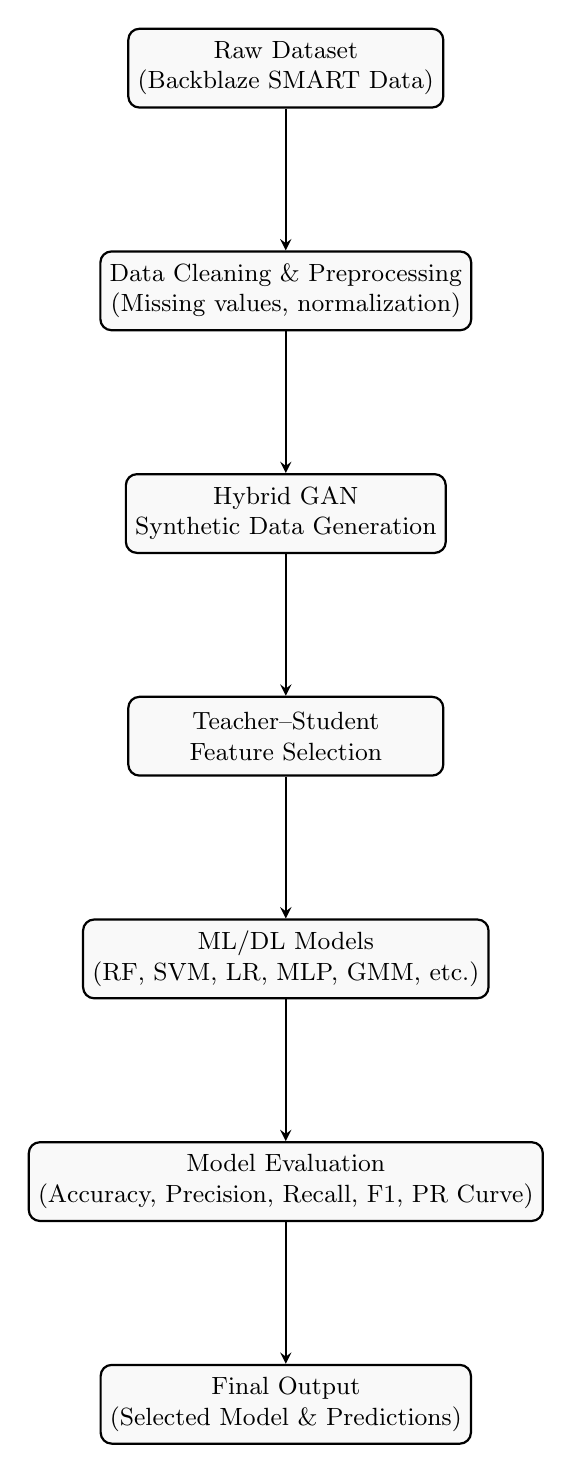
\begin{tikzpicture}[
                node distance=1.8cm,
                every node/.style={font=\small},
                process/.style={rectangle, rounded corners, minimum width=4cm, minimum height=1cm, draw=black, thick, fill=gray!5, align=center},
                arrow/.style={thick,->,>=stealth}
            ]
            
                % Nodes
                \node (input) [process] {Raw Dataset\\(Backblaze SMART Data)};
                \node (clean) [process, below=of input] {Data Cleaning \& Preprocessing\\(Missing values, normalization)};
                \node (gan) [process, below=of clean] {Hybrid GAN\\Synthetic Data Generation};
                \node (feat) [process, below=of gan] {Teacher–Student\\Feature Selection};
                \node (models) [process, below=of feat] {ML/DL Models\\(RF, SVM, LR, MLP, GMM, etc.)};
                \node (eval) [process, below=of models] {Model Evaluation\\(Accuracy, Precision, Recall, F1, PR Curve)};
                \node (out) [process, below=of eval] {Final Output\\(Selected Model \& Predictions)};
                
                % Arrows
                \draw [arrow] (input) -- (clean);
                \draw [arrow] (clean) -- (gan);
                \draw [arrow] (gan) -- (feat);
                \draw [arrow] (feat) -- (models);
                \draw [arrow] (models) -- (eval);
                \draw [arrow] (eval) -- (out);
            
            \end{tikzpicture}
            
            \caption{End-to-End Workflow of the Hard Drive Failure Prediction System}
        \end{figure}
    \caption{Model Accuracy}
\end{figure}

\newpage

% ============================================================
% Chapter 5
% ============================================================

\section{Findings, Recommendations and Conclusion}

\subsection{Findings}
\lipsum[9]

\subsection{Recommendations}
\lipsum[10]

\subsection{Conclusion}
\lipsum[11]

\newpage

% ============================================================
% Chapter 6
% ============================================================

\section{Future Scope}

\lipsum[12]

\newpage

% ============================================================
% Glossaries
% ============================================================

\printglossaries
\addcontentsline{toc}{section}{List of Abbreviations}
\newpage

% ============================================================
% References
% ============================================================

% \begin{thebibliography}{99}
%     \addcontentsline{toc}{section}{References}

%     \bibitem{Ileberi2022}  
%     E. Ileberi, Y. Sun, Z. Wang, “A machine learning based credit card fraud detection using the GA algorithm for feature selection,” *Journal of Big Data*, vol. 9, no. 1, p. 24, 2022. DOI: 10.1186/s40537-022-00573-8.
    
%     \bibitem{BinSulaiman2022}  
%     R. Bin Sulaiman, V. Schetinin, P. Sant, “Review of Machine Learning Approach on Credit Card Fraud Detection,” *Human-Centric Intelligent Systems*, vol. 2, no. 10, pp. 55–68, 2022. DOI: 10.1007/s44230-022-00004-0.
    
%     \bibitem{IJARSCT22301}  
%     [Author(s)], “[Title of the paper from PDF],” *International Journal of Advanced Research in Science, Communication and Technology (IJARSCT)*, [year]. Available: \url{https://ijarsct.co.in/Paper22301.pdf}.
    
%     \bibitem{SSRG_IJECE_665}  
%     [Author(s)], “A Machine Learning Based Approach for the Fraud Detection in Credit Card Transactions,” *SSRG International Journal of Electronics and Communication Engineering (IJECE)*, Paper Id 665, [year]. Available: \url{https://www.internationaljournalssrg.org/IJECE/paper-details?Id=665}.
    
%     \bibitem{FrontiersFrai2025}  
%     [Author(s)], “[Title],” *Frontiers in Artificial Intelligence*, 2025. DOI: 10.3389/frai.2025.1643292.
    
%     \bibitem{ChuEnsemble2023}  
%     Y. B. Chu, Z. M. Lim, B. Keane, P. H. Kong, A. R. Elkilany, O. H. Abusetta, “Credit Card Fraud Detection on Original European Credit Card Holder Dataset Using Ensemble Machine Learning Technique,” *Cyber Security Journal*, vol. 5, no. 1, pp. 33–46, 2023. URL: \url{https://cyberir.mit.edu/site/credit-card-fraud-detection-original-european-credit-card-holder-dataset-using-ensemble-machine/}.
    
%     \bibitem{AIP_ACP_CreditCard}  
%     [Author(s)], “Credit-card fraud detection using machine learning,” *AIP Advances in Computational Physics*, vol. 1, no. 1, p. 020030, [year]. DOI: 10.1063/1.3351466.
    
%     \bibitem{SD_Paper1}  
%     [Author(s)], “[Title],” *[Journal Name]*, [volume], [pages], [year]. DOI: [DOI of the ScienceDirect paper].
    
%     \bibitem{SD_Paper2}  
%     [Author(s)], “[Title],” *[Journal Name]*, [volume], [pages], 2024. DOI: [DOI of the second ScienceDirect paper].
    
%     \bibitem{Plakandaras2022}  
%     V. Plakandaras, *et al.*, “Credit Card Fraud Detection with Automated Machine Learning Systems,” *Applied Artificial Intelligence*, vol. 36, no. 1, [pages], 2022. DOI: 10.1080/08839514.2022.2086354.

% \end{thebibliography}

\newpage
\printbibliography

% ============================================================
% Document End
% ============================================================

\end{document}
